%%%%%%%%%%%%%%%%%%%%%%%%%%%%%%%%%%%%%%%%%%%%%%%%%%%%%%%%%%%%%%%%%%%%%%%%%%%%%%%%%%%%%%%%%%%
\section{Discussion}\label{sec:discussion}

\subsection{Solution}\label{sec:solution}

The solution to the differential equation \eqref{eq:susyConditionTheta} is:
\begin{equation}\label{eq:susyConditionSolution}
\boxed{\sin\theta(c) = L \sqrt{c^2-1}; \quad 1 < c \leq \sqrt{1+L^{-2}}, \quad L < 1},
\end{equation}
where $L$ is an integration constant, which is proportional to the mass of the fundamental matter (or quark) field in the dual field theory, as we explain next. The upper bound of $c$ is set by the maximum of the sine.

Near the boundary, $c \approx 1 + z^2/2$, the solution behaves as
\begin{equation} \label{eq:thetaExpanded}
 \theta(z) \approx L \, z + \left(\frac{L}{8} +\frac{L^3}{6} \right) \, z^3 + O(z^5).
\end{equation} 
Notice that only at the leading order large $L$ expansion, our solution reduces to the exact form found in the $AdS_5 \times S^5$ background, see \cite{Karch:2002sh} and \cite{Karch:2005ms}, i.e.
\begin{equation}
 \sin\theta(z)_\text{AdS} = L z,
\end{equation}
with the asymptotic expansion
\begin{equation}
\theta(z)_\text{AdS} \approx L z + \frac{L^3}{6} z^3 + O(z^5).
\end{equation}

As \cite{Karch:2005ms} explains, in the flat embedding space limit, this embedding describes a planar D-brane located at a constant distance $L$ away from the stack of $N$ D3-branes:
\begin{equation}
 L = \lim_{z \rightarrow 0 } \frac{1}{z} \sin\theta(z),
\end{equation}
and this distance is proportional to the quark mass $m$:
\begin{equation}
 L = \dfrac{m}{2 \pi l_s^2}.
\end{equation}


Figures in \ref{fig:vielbeins} show the vielbeins of the induced metric at the solution, from which we learn how the geometry of the embedding looks like at different values of $c$. First, observe the divergence at the horizon $c_{max}=\sqrt{1+L^{-2}}$. This is the location of the well-known enhançon locus, at $\theta = \pi/2$, see \cite{Buchel:2000cn} and \cite{Evans:2000ct}. The spheroid is undeformed at the boundary $c=1$, and becomes squashed until it vanishes at the enhançon. 

\begin{figure}[t!]
\begin{center}
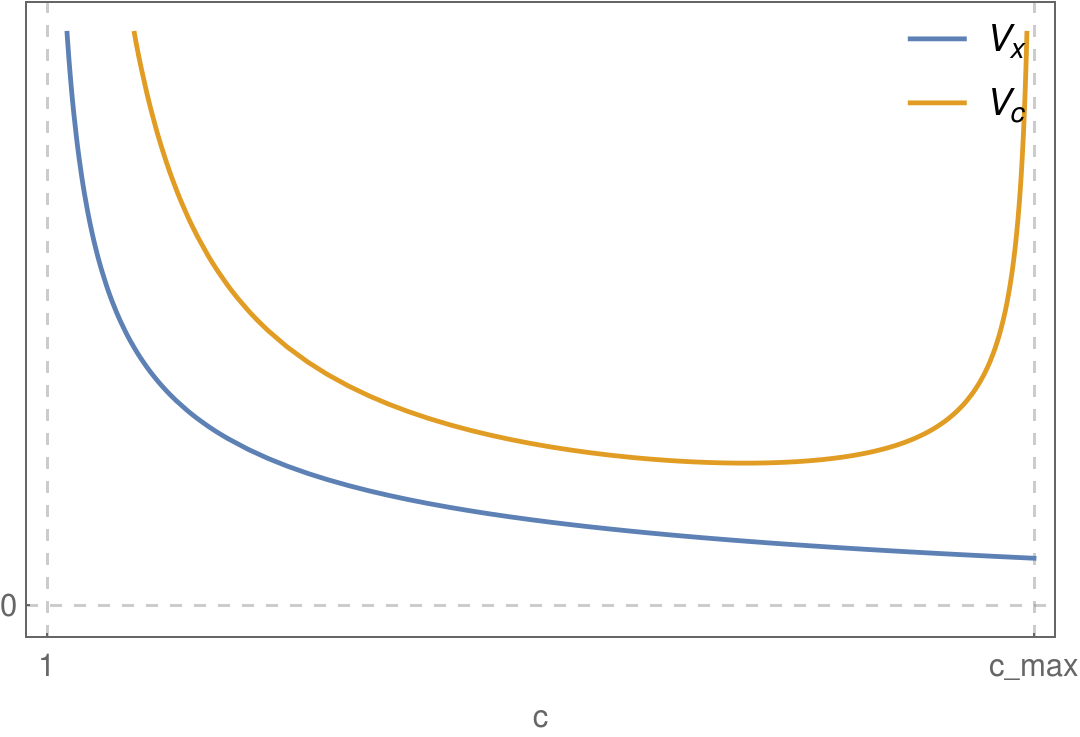
\includegraphics[width=0.6\textwidth]{pictures/vxvcb.png}
\end{center}
\vspace{0.05mm}
\begin{center}
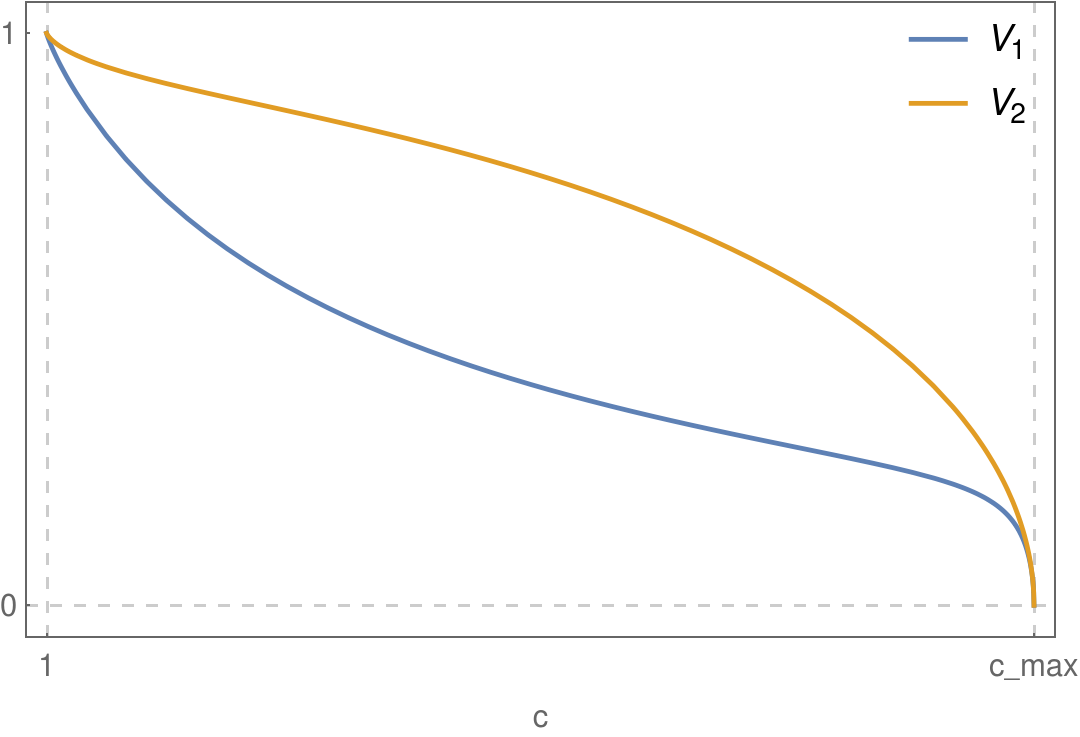
\includegraphics[width=0.6\textwidth]{pictures/v1v2b.png}
\end{center}
\caption{\label{fig:vielbeins} The vielbeins of the induced metric for the allowed values of $c$.}
\end{figure}



%%%%%%%%%%%%%%%%%%%%%%%%%%%%%%%%%%%%%%%%%%%%%%%%%%%%%%%%%%%%%%%%%%%%%%%%%%%%%%%%%%%%%%%%%%%%%%%%%
\subsection{Action}


The D7-brane action \eqref{eq:DbraneAction} for our configuration \eqref{eq:ansatz} can be written as:
\begin{align} \label{eq:ActionWithTheta'}
 S  = & -T_7 \int_\mathcal{M} d^8\xi \, e^{-P[\Phi] } v_x^4 v_c v_1 v_2^2 \sqrt{1+\frac{v_\theta^2}{v_c^2}\theta'(c)^2}  \nonumber \\
      & + T_7\int _\mathcal{M} P[C_{(8)}],
\end{align}
or more explicitly, using the solution \eqref{eq:susyConditionTheta}, as:
\begin{align}\label{eq:ActionWithTheta}
 S = & -T_7 \int_\mathcal{M} d^8\xi \, \dfrac{c A(c) \cos^3\theta (c) \sqrt{X_1(c, \theta(c))}}{\left(c^2-1\right)^3} \sqrt{1+ c A(c) \tan^2\theta(c)} \nonumber \\
     & +T_7\int _\mathcal{M} d^8\xi \, \dfrac{A(c)^2 \cos^4\theta(c)}{4 \left(c^2-1\right)^2}.
\end{align}
The explicit form of the Wess-Zumino term is calculated below.

\subsubsection{Wess-Zumino term}
The $P[C_{(8)}]$ term was deemed vanishing in \cite{Albash:2011nw} and \cite{Evans:2005ti}. Their argument did not consider the dilaton factor in the string frame that affects the Hodge star operation while deriving $C_{(8)}$, which in our scenario is
\begin{equation}
 dC_{(8)} = \ast dC_{(0)}.
\end{equation}
The dilaton term from the string frame effectively cancels the factor that vanishes at $\phi_0$, leading to a finite value for the pullback of this potential. We decided to compute it explicitly, and the full result is given in the appendix \ref{sec:backgroundFields}. We can quickly see that it is non-zero for our ansatz for $\phi$ in \eqref{eq:ansatz}. However, $P[C_{(8)}]$ term can be much simpler, as we will see now. First, we can show that:
\begin{equation}\label{eq:C8id}
 [d C_{(8)}]_{\phi_0} = d [C_{(8)}]_{\phi_0}.
\end{equation}
The left-hand-side is simply
\begin{equation}
 [d C_{(8)}]_{\phi_0}  = \dfrac{A^2 \sin\theta \cos^3(\theta)}{\left(c^2-1\right)^2} 
\sigma_1 \wedge \sigma_2 \wedge \sigma_3 \wedge dc  \wedge dx_0 \wedge dx_1 \wedge dx_2 \wedge dx_3 \wedge d\theta,
\end{equation}
and, via \eqref{eq:C8id}, we can integrate the above expression over $\theta$ and obtain:
\begin{equation}
[C_{(8)}]_{\phi_0} = \dfrac{A^2 \cos^4\theta}{4 \left(c^2-1\right)^2} \sigma_1 \wedge \sigma_2 \wedge \sigma_3 \wedge dc \wedge dx_0 \wedge dx_1 \wedge dx_2 \wedge dx_3.
\end{equation}
The full pullback is obtained by just replacing $\theta$ by $\theta(c)$.




%%%%%%%%%%%%%%%%%%%%%%%%%%%%%%%%%%%%%%%%%%%%%%%%%%%%%%%%%%%%%%%%%%%%%%%%%%%%%%%%%%%%%%%%%%%%%%%%%

\subsection{Equation of motion}

As a consistency check for our results, the equation of motion from the action \eqref{eq:ActionWithTheta'} is fulfilled with the solution \eqref{eq:susyConditionTheta}. In particular, 
\begin{align}\label{eq:eom}
-\left.EL[\mathcal{L}_{DBI}]\right|_\text{solution} = EL[\mathcal{L}_{WZ}] = \dfrac{A^2 \sin\theta \cos^3(\theta)}{\left(c^2-1\right)^2},
\end{align}
where $EL[\cdot]$ is the Euler-Lagrange operator:
\begin{equation}
 EL[\mathcal{L}] = 
 \left(\dfrac{\pd }{\pd \theta(c)} -\dfrac{\pd }{\pd c}  \dfrac{\pd }{\pd \theta'(c)} \right) \mathcal{L}.
\end{equation}
Therefore, \eqref{eq:eom} is another proof for the non-vanishing WZ term.



\subsection{Holographic renormalization}
In this subsection, we are going to renormalize the action and check that the chiral condensate is zero, as we expect from a supersymmetry embedding.

The fully explicit on-shell action evaluated at the solution \eqref{eq:susyConditionSolution} is:
\begin{align}\label{eq:ActionAtSolution}
 S_\text{reg} = -T_7 V \int_{1 + \epsilon^2/2}^{c_\text{max}} d c \, 
 &\left[-\frac{c A(c)}{\left(c^2-1\right)^3} -\frac{A(c)^2}{4 \left(c^2-1\right)^2} \right. \nonumber\\
 &-\frac{L^2 A(c) \left(\left(c^2+1\right) A(c)-4 c\right)}{2 \left(c^2-1\right)^2} \nonumber\\
 &+\left.\frac{L^4 A(c) \left(3 c^2 A(c)+A(c)-4 c\right)}{4 \left(c^2-1\right)}\right],
\end{align}
where $c_\text{max}$ is the upper bound shown in \eqref{eq:susyConditionSolution}, and $V$ denotes the volume of the 4-dimensional Minkowski space times the 3-sphere. Notice that the action is divergent near the boundary, thus, we regularized it by adding a regulator $\epsilon>0$ in the lower integration limit. The divergent terms are explicitly:
\begin{align} \label{eq:Sdiv}
 S_\text{div} = T_7 V 
        \left[ \frac{1}{4 \epsilon ^4} +\frac{1+\log \left(\epsilon/2\right)}{2 \epsilon ^2}-\frac{L^2}{2 \epsilon ^2}-\frac{ \log ^2\left(\epsilon/2\right)}{4}+\frac{\log (\epsilon )}{8} \right].
\end{align}

Notice that the divergent terms independent of $L$ must come from the integration of the first line of \eqref{eq:ActionAtSolution}, where the first term comes from DBI and the second from WZ. Similarly, the $L^2$ divergent term comes from the second line of \eqref{eq:ActionAtSolution}. 
We propose the following counterterms:
\begin{align}\label{eq:counterterms}
 S_\text{CT} =  -T_7 V \left[ 
  \frac{1}{4} \left(\frac{1}{\epsilon ^4}-\frac{1}{2 \epsilon ^2}\right) f(\epsilon)
   -\frac{1}{2}\left(\frac{1}{\epsilon ^4}+\frac{2}{3 \epsilon ^2}\right) \theta (\epsilon)^2 + \frac{3}{8 \epsilon^4} \theta (\epsilon)^4
   \right],
\end{align}
where the scalar field expansion is found in \eqref{eq:thetaExpanded}, and
$f(\epsilon)$ consists of the divergent terms of the expression 
\begin{equation}
A(c)-A(c)^2 c - 2 c + 3 A(c) c^2,
\end{equation}
evaluated at $c=1+\epsilon^2/2$. 


Although the divergences \eqref{eq:Sdiv} can be obtained by first expanding the on-shell Langragian and then integrate, we remark that this process cannot give us constant terms. We must know these, since by introducing $\theta(\epsilon)^2$ term, we do introduce additional finite terms. Therefore, we performed the exact integration, where the results are found in the appendix \ref{sec:integrate-action}. The finite counterterms we introduced, which are the second term of $\theta(\epsilon)^2$ and the $\theta(\epsilon)^4$ term in \eqref{eq:counterterms} are fixed to cancel these UV constant terms.


Equation \eqref{eq:counterterms} resembles, but does not exactly match, the counterterms derived for general asymptotic AdS spaces for the D7-brane \cite{Karch:2005ms}:
\begin{align*}
& L_{1}=-\frac{1}{4} \sqrt{\gamma} \\
& L_{4}=\frac{1}{2} \sqrt{\gamma} \theta(\epsilon)^2 \\
& L_{f}= -\frac{5}{12}\sqrt{\gamma} \theta(\epsilon)^4,
\end{align*}
where $\gamma$ here denotes the regulator hypersurface metric. We suspect our geometry is not covered by this general study, due to the logarithmic divergence appearing already at the next-to-leading order $\epsilon$-expansion for the metric, coming from $A(c)$. The finite counterterm $L_f$ also removes the IR finite term, while our quartic term does not. That is because our IR terms, namely from the upper-limit of the integral in \eqref{eq:ActionAtSolution}, are highly non-trivial functions of $L$. We do not believe a simple counterterm in terms of the scalar field can do the job. \comment{Do we expect the action to be always zero because of SUSY? Our D3-brane action was non-zero, though its DBI+WZ=0.}

\subsubsection*{Large L}
As we discussed in \ref{sec:solution}, our embedding matches with the one in the $AdS_5 \times S^5$ background at large $L$. At this limit, $c_{\max }\approx 1+ 1/(2 L^{2})$, and the IR contribution to the action reduces to $-L^4/6$. Hence, it can be canceled by a quartic field counterterm, thus:
\begin{align}\label{eq:countertermsLargeL}
 S_{\text{CT}, L\gg 1} =  -T_7 V \left[ 
  \frac{1}{4} \left(\frac{1}{\epsilon ^4}-\frac{1}{2 \epsilon ^2}\right) f(\epsilon)
   -\frac{1}{2}\left(\frac{1}{\epsilon ^4}+\frac{2}{3 \epsilon ^2}\right) \theta (\epsilon)^2 + \frac{5}{24 \epsilon^4} \theta (\epsilon)^4
   \right].
\end{align}

The renormalized action, defined as
\begin{equation}
 S_\text{ren} = \lim_{\epsilon\rightarrow 0} (S_\text{reg}-S_\text{CT}),
\end{equation}
is hence exactly zero for the large $L$ case. Consequently, the chiral condensate, sourced by $L$, also vanishes:
\begin{equation} 
\langle O \rangle = \frac{\delta S_\text{ren}}{\delta L} = 0. 
\end{equation}




 




